\chapter{}

\section{}

Abbildung \ref{fig:7:kennlinie} zeigt die Drehzahl-Drehmomentkennlinie, die beim Versuch im Labor Antriebstechnik aufgenommen wurde. Dabei befinden sich die blauen Linien im Ankerstellbereich und die roten im Feldschwächbereich.

\section{}
Nun soll anhand der in Aufgabe 4 ermittelten Parametern eine Drehzahl-Drehmomentkennlinie berechnet werden. Dabei wird in die Formel (\ref{eq:7:N}) folgende Werte eingetragen:
\begin{center}
	$ U_{A} = 60V $ \hspace{1.5cm}	$ R_{A} = 6.4\Omega $ \hspace{1.5cm}	$ c_{E}\Psi = 2.919Vs$
\end{center}
\begin{equation}
	N = \frac{U_{A}}{c_{E}\Psi} - \frac{2\pi R_{A}}{c_{E}^{2}\psi^{2}}M_{Mi}
	\label{eq:7:N}
\end{equation}
Die berechnete Kennlinie wird in Abbildung \ref{fig:7:kennlinie} in grün aufgetragen. Dabei ist zu erkennen, dass mit steigenden Lastmoment die (berechnete) Drehzahl sich weniger verringert als bei den gemessenen Linien. Dies ist auf unvermeidbare Verluste im Prüfstand zurückzuführen.

\begin{figure}[h]
	\centering 
	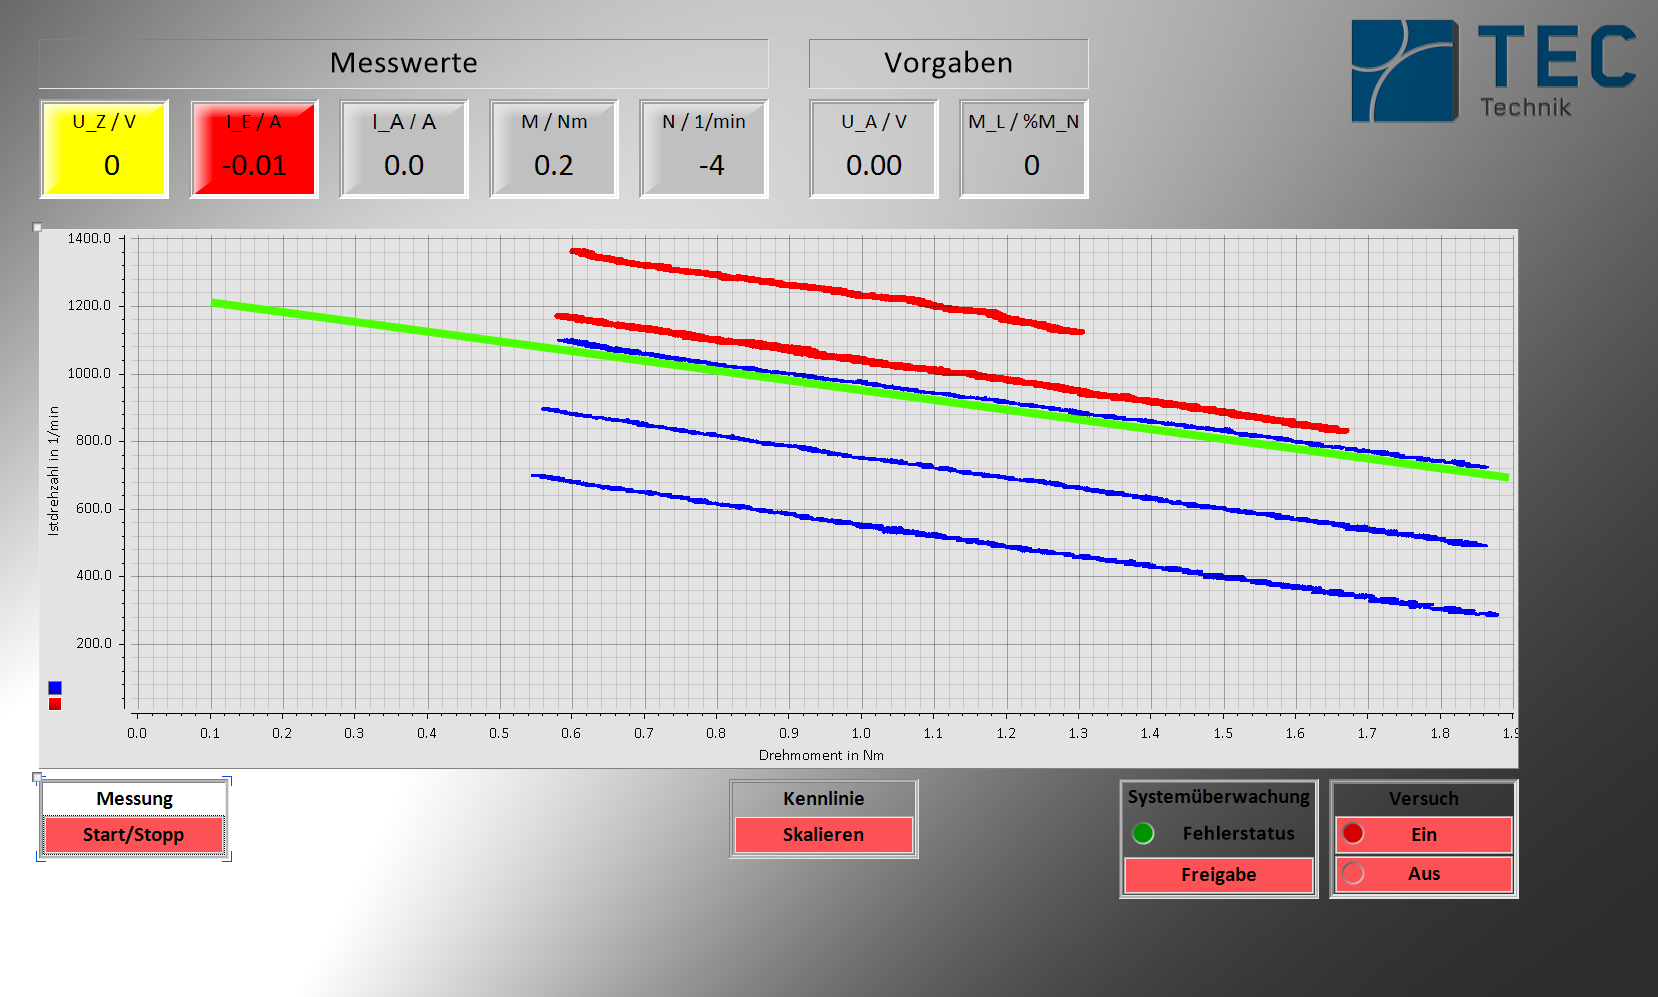
\includegraphics[width=\textwidth]{./bilder/kennlinie.png}
	\caption{Drehzahl-Drehmomentkennlinie aus dem Labor Antriebstechnik}
	\label{fig:7:kennlinie}
\end{figure}